\chapter[Log Correlated Fields]{Log Correlated Fields: Selberg's Central Limit Theorem, Maxima and Multiplicative Chaos}\label{ch:09b}

In 1946 Selberg proved that the logarithm of the Riemann zeta function on the critical line is asymptotically Gaussian: if $t$ is chosen at random between $T$ and $2T$, then $\log|\zeta(\frac12+it)|$ is approximately normal with mean zero and variance $\frac12\log\log T$ \cite{selberg1946}. The variance grows, but so slowly that at every height a computer will ever reach it is a single digit number, and for six decades the theorem was read as a statement about the value at one random point, a part of the value distribution theory of Chapter~\ref{ch:09}. Its modern meaning emerged when Fyodorov, Hiary and Keating \cite{fhk2012} looked at $t\mapsto\log|\zeta(\frac12+it)|$ on a whole window of unit length. Two points at distance $h$ share the primes $p$ with $\log p<1/h$ and see independent phases for the others, so for $1/\log T\le h\le1$ the covariance of the field is about $\frac12\log(1/h)$: the field is \emph{log correlated}, the same structure that governs branching random walks, the two dimensional Gaussian free field, and the characteristic polynomials of random unitary matrices. From that structure they predicted the maximum over a unit window up to a bounded random error, and Arguin, Bourgade and Radziwi\l\l\ have since proved the prediction to that accuracy; the law of the error is still open. The exponential of a log correlated field is a multiplicative chaos, and Saksman and Webb showed that the zeta function on a random window converges in law, as a random generalised function, to a complex multiplicative chaos times a smooth random function. Harper found the same chaos, at its critical point, inside the partial sums of random multiplicative functions. This chapter develops these ideas for $\zeta$ and for the discriminant form $\Delta$, tests them on our own computations of $L(s,\Delta)$, and connects them with the Thorin and extreme value representations of the chapters that follow.

\paragraph{Conventions.} We write $L(s,\Delta)=\sum_n\tau(n)n^{-s}$ in the classical normalisation of Chapter~\ref{ch:02}, so that the centre is $s=6$ and the critical line is $6+it$. Put $\lambda(n)=\tau(n)/n^{11/2}$ and $\lambda(p)=x_p=2\cos\theta_p$ with $\theta_p\in[0,\pi]$ (Deligne). Then
\[
L(6+it,\Delta)=\prod_p\Bigl[\bigl(1-e^{i\theta_p}p^{-\frac12-it}\bigr)\bigl(1-e^{-i\theta_p}p^{-\frac12-it}\bigr)\Bigr]^{-1}
\]
formally, and $\log|L(6+it,\Delta)|$ is $\log|L(\frac12+it)|$ in the unitary normalisation used in Chapter~\ref{ch:09}. The completed function is $\Lambda(s,\Delta)=(2\pi)^{-s}\Gamma(s)L(s,\Delta)$, and the Hardy function
\[
Z_\Delta(t)=e^{i\vartheta(t)}L(6+it,\Delta),\qquad\vartheta(t)=\arg\bigl((2\pi)^{-it}\Gamma(6+it)\bigr),
\]
with $\vartheta$ continuous and $\vartheta(0)=0$, is real for real $t$, and $|Z_\Delta(t)|=|L(6+it,\Delta)|$. The zeros of $L(s,\Delta)$ near height $t$ have density $\frac1\pi\log\frac{t}{2\pi}$, twice that of $\zeta$, because the analytic conductor is of size $t^2$.

\section{Selberg's central limit theorem}\label{sec:09bselberg}

\begin{theorem}[Selberg \cite{selberg1946}]\label{thm:09bselberg}\index{Selberg central limit theorem}
Let $t$ be uniformly distributed on $[T,2T]$. As $T\to\infty$,
\[
\frac{\log\zeta(\frac12+it)}{\sqrt{\frac12\log\log T}}\Longrightarrow X+iY,
\]
with $X$ and $Y$ independent standard normal variables. In particular $\log|\zeta(\frac12+it)|/\sqrt{\frac12\log\log T}$ is asymptotically standard normal.
\end{theorem}

Selberg's original account is brief, and a detailed proof was written out by Tsang \cite{tsang1984}. The heuristic behind it is the random model of Chapter~\ref{ch:09}. Formally $\log\zeta(\frac12+it)=\sum_p p^{-1/2-it}+O(1)$, and for $t$ uniform on $[T,2T]$ the phases $p^{-it}$, $p\le T^{\varepsilon}$, behave like independent uniform variables on the circle, because a monomial $\prod p^{-ik_pt}$ averages to almost zero over $[T,2T]$ unless it is trivial. The real part of $p^{-1/2-it}$ then has variance $\frac1{2p}$, and the variance of the prime sum over $p\le x$ is $\frac12\sum_{p\le x}\frac1p=\frac12\log\log x+O(1)$ by Mertens' theorem. The difficulty, which occupies the whole proof, is that the Dirichlet series diverges on the line and that zeros of $\zeta$ make $\log|\zeta|$ singular.

\subsection{The variance for the discriminant form}

For $\Delta$ the prime sum is $\operatorname{Re}\sum_p\lambda(p)p^{-1/2-it}$, whose variance in the random phase model is $\frac12\sum_{p\le x}\lambda(p)^2/p$. Its growth is controlled by the Rankin Selberg convolution, exactly as the positivity of Chapter~\ref{ch:09} was.

\begin{lemma}\label{lem:09brs}
There is a constant $B_\Delta$ such that $\sum_{p\le x}\lambda(p)^2/p=\log\log x+B_\Delta+o(1)$.
\end{lemma}

\begin{proof}
The Hecke relation $\tau(p)^2=\tau(p^2)+p^{11}$ gives $\lambda(p)^2=1+\lambda(p^2)$, and $\lambda(p^2)=e^{2i\theta_p}+1+e^{-2i\theta_p}$ is the coefficient at $p$ of the symmetric square $L(s,\Sym^2\Delta)$ in the unitary normalisation. Since $\Delta$ has no complex multiplication, $\Sym^2\Delta$ is a cuspidal automorphic representation of $\GL_3$ by Gelbart and Jacquet \cite{gelbartjacquet1978}, so $L(s,\Sym^2\Delta)$ is entire and does not vanish on $\operatorname{Re}s=1$ \cite{jacquetshalika1976}. A zero free region of de la Vall\'ee Poussin type (Chapter 5 of \cite{iwanieckowalski2004}; a possible exceptional real zero $\beta<1$ of this single function only contributes $O(x^\beta)$) gives $\sum_{p\le x}\lambda(p^2)\log p=O(x/\log^2x)$, and partial summation shows that $\sum_p\lambda(p^2)/p$ converges. Mertens' theorem $\sum_{p\le x}1/p=\log\log x+M+o(1)$ finishes the proof, with $B_\Delta=M+\sum_p\lambda(p^2)/p$.
\end{proof}

So the variance of the prime sum for $\Delta$ is again $\frac12\log\log x$ to leading order; the degree of the $L$ function does not enter, because the Rankin Selberg function $L(s,\Delta\times\Delta)=\zeta(s)L(s,\Sym^2\Delta)$ has a simple pole at $s=1$. The constant, however, is far from zero. From $\tau(p)$ for all $p\le10^5$, computed with PARI/GP for this book, we find $B_\Delta\approx-0.688$: the partial sums $\sum_{p\le x}\lambda(p)^2/p-\log\log x$ are $-0.6854$ and $-0.6874$ at $x=10^4$ and $10^5$, and the limit, computed from $L(1,\Sym^2\Delta)$ by the method of Exercise~\ref{ex:09bmertens}, is $-0.6879$. The value is driven by the small primes: $\lambda(2)^2=0.281$ and $\lambda(3)^2=0.358$, against the Sato Tate average $1$.

\begin{theorem}[Selberg; Bombieri and Hejhal]\label{thm:09bselbergdelta}
Assume the Riemann hypothesis for $L(s,\Delta)$. For $t$ uniform on $[T,2T]$,
\[
\frac{\log|L(6+it,\Delta)|}{\sqrt{\frac12\log\log T}}\Longrightarrow N(0,1),
\]
and the same holds for the argument, jointly, with independent limits.
\end{theorem}

Selberg announced, under a zero density hypothesis, the central limit theorem for the class of Dirichlet series that now bears his name \cite{selberg1992}, and Bombieri and Hejhal \cite{bombierihejhal1995} proved joint versions for several $L$ functions under hypotheses on their zeros, which they used to study zeros of linear combinations of Euler products. We state the theorem under the Riemann hypothesis for $L(s,\Delta)$, under which the zero density hypotheses of both works hold trivially. The short proof described next needs no zero density estimate at all. Its one input specific to $\zeta$ is the twisted second moment of Step~2, and Radziwi\l\l\ and Soundararajan remark that the analogous estimate in degree two can be obtained from bounds for shifted convolution sums; that would give the statement for $\log|L(6+it,\Delta)|$ without the Riemann hypothesis, but we know of no published account for $\Delta$, so we keep the hypothesis.

\subsection{The proof of Radziwi\l\l\ and Soundararajan}

Radziwi\l\l\ and Soundararajan \cite{radziwillsound2017} gave a proof of Theorem~\ref{thm:09bselberg} that fits on a few pages. We sketch it for $\zeta$; for $\Delta$ one replaces $p^{-s}$ by $\lambda(p)p^{-s}$, uses Lemma~\ref{lem:09brs} for the variance, and needs the degree two analogue of Step~2 discussed above.

\begin{proof}[Sketch]
Put $W=(\log\log\log T)^4$, $\sigma_0=\frac12+W/\log T$, $X=T^{1/(\log\log\log T)^2}$, and $\mathcal{P}(s)=\sum_{2\le p\le X}p^{-s}$.

Step 1 (moments of the prime sum). For a Dirichlet polynomial $A(s)=\sum_{n\le N}a_nn^{-s}$ with $N\le T$ one has $\frac1T\int_T^{2T}|A(\sigma+it)|^2dt=\sum_n|a_n|^2n^{-2\sigma}(1+O(N/T))$. Expanding $\operatorname{Re}\mathcal{P}(\sigma_0+it)^k$ for $k$ up to a slowly growing bound gives Dirichlet polynomials of length $X^k\le T^{o(1)}$, and the diagonal terms reproduce the moments of a sum of independent random variables $\operatorname{Re}(U_pp^{-\sigma_0})$ with $U_p$ uniform on the circle. Hence $\operatorname{Re}\mathcal{P}(\sigma_0+it)$ has asymptotically the moments of $N(0,\frac12\sum_{p\le X}p^{-2\sigma_0})$, and the variance is $\frac12\log\log T+O(\log\log\log T)$.

Step 2 (off the line, a mollifier). Let $\mathcal{M}(s)$ be the Dirichlet polynomial obtained by truncating the Taylor series of $\exp(-\mathcal{P}(s))$ suitably. A twisted second moment computation shows that $\frac1T\int_T^{2T}|1-\zeta(\sigma_0+it)\mathcal{M}(\sigma_0+it)|^2dt$ tends to zero. On the set where $|\mathcal{P}(\sigma_0+it)|$ is not too large, $\mathcal{M}=\exp(-\mathcal{P})(1+o(1))$, so $\log|\zeta(\sigma_0+it)|=\operatorname{Re}\mathcal{P}(\sigma_0+it)+o(1)$ outside a set of measure $o(T)$.

Step 3 (back to the line). Using the Hadamard factorisation, $\log|\zeta(\sigma_0+it)|-\log|\zeta(\frac12+it)|$ is a sum over zeros $\rho$ of $\log|(\sigma_0+it-\rho)/(\frac12+it-\rho)|$ plus a smooth term, and integrating over $t$ gives
\[
\int_T^{2T}\bigl|\log|\zeta(\tfrac12+it)|-\log|\zeta(\sigma_0+it)|\bigr|\,dt\ll(\sigma_0-\tfrac12)\,T\log T=WT .
\]
Hence the difference is $O(W)$ on average, which is $o(\sqrt{\log\log T})$.

Step 4. Combining the three steps, $\log|\zeta(\frac12+it)|$ equals $\operatorname{Re}\mathcal{P}(\sigma_0+it)+o(\sqrt{\log\log T})$ outside a set of measure $o(T)$, and Step 1 gives the Gaussian limit. This is the real part of the theorem, and it is all that Radziwi\l\l\ and Soundararajan treat. The imaginary part does not follow verbatim, since knowing that $\zeta\mathcal{M}$ is close to $1$ fixes $\operatorname{Im}\log\zeta(\sigma_0+it)$ only modulo $2\pi$; its Gaussian limit goes back to Selberg's computation of the moments of $S(t)=\pi^{-1}\arg\zeta(\frac12+it)$ \cite{selberg1946}.
\end{proof}

The arithmetic enters through mean values: of Dirichlet polynomials in Step 1, the precise sense in which the $p^{-it}$ are independent, and of $\zeta$ twisted by a short Dirichlet polynomial in Step 2. The analytic content is the passage from $\sigma_0$ to the line across the zeros.

\subsection{Finite height: a heavy left tail}\label{sec:09btail}

The central limit theorem is a statement about $\log\log T\to\infty$, and at any accessible height the distribution of $\log|L|$ is visibly not normal. The most visible departure comes from the zeros. Near a simple zero $\gamma$ of $Z_\Delta$, $\log|Z_\Delta(t)|=\log|t-\gamma|+\log|Z'_\Delta(\gamma)|+O(|t-\gamma|)$, which tends to $-\infty$, while large positive values require many primes to conspire.

\begin{proposition}[Exponential left tail; this book]\label{prop:09blefttail}
Let $f$ be real analytic on a neighbourhood of $[a,b]$, with finitely many zeros $\gamma_1,\dots,\gamma_r$ in $(a,b)$, all simple, and none at $a$ or $b$. Then, as $x\to\infty$,
\[
\Bigl|\bigl\{t\in[a,b]:\log|f(t)|<-x\bigr\}\Bigr|=2e^{-x}\sum_{j=1}^r\frac{1}{|f'(\gamma_j)|}+O(e^{-2x}).
\]
\end{proposition}

\begin{proof}
Away from the zeros $|f|$ is bounded below by a positive constant, so for large $x$ the set lies in small neighbourhoods of the $\gamma_j$. Near $\gamma_j$ write $f(t)=f'(\gamma_j)(t-\gamma_j)(1+g_j(t))$ with $g_j$ analytic and $g_j(\gamma_j)=0$. The set $\{|f(t)|<e^{-x}\}$ near $\gamma_j$ is an interval with endpoints $\gamma_j\pm e^{-x}/|f'(\gamma_j)|\,(1+O(e^{-x}))$, whose length is $2e^{-x}/|f'(\gamma_j)|+O(e^{-2x})$.
\end{proof}

Applied to $f=Z_\Delta$ on a window $[T,2T]$ whose zeros are simple, the proposition says that the empirical law of $\log|L(6+it,\Delta)|$ has a left tail $\Prob(\log|L|<-x)\approx Ce^{-x}$, exponential with rate one, while a normal law of variance $V$ has tail $\exp(-x^2/(2V))$. In standard units the exponential tail is $\exp(-\sqrt V\,y)$, heavier than Gaussian for every finite $V$; it disappears from the limit only because $\sqrt V\to\infty$. The right tail is different: it is governed by the large deviations of the prime sum, and it is close to Gaussian in the range of the central limit theorem.

\paragraph{Data.} For this book we evaluated $\log|L(6+it,\Delta)|$ with PARI/GP at $50{,}000$ points $t\in[500,2500)$ with step $0.04$. The sample mean is $0.0020$ and the sample variance is $1.5265$, against $\frac12\log\log t=0.9948$ at the midpoint $t=1500$. The skewness is $-1.135$ and the excess kurtosis is $2.493$, and a Kolmogorov Smirnov test of the standardised values against $N(0,1)$ rejects decisively: the distance is $0.069$. Neighbouring values are strongly dependent, so we quote no $p$ value for all $50{,}000$ of them; each of the $15$ subsamples of every $15$th value, spaced by about one mean zero spacing, has a nominal $p<10^{-10}$. Figure~\ref{fig:09bclt} shows the shape of the departure: a long left tail, and a bulk shifted to the right with a right tail lighter than the normal one. This does not conflict with Theorem~\ref{thm:09bselbergdelta}, which is a limit statement: at height $10^3$ the normal law describes the centre of the distribution but not its tails, and the variance is about one and a half times its leading asymptotic. Section~\ref{sec:09bhybrid} accounts for the variance.

\begin{figure}[t]\centering
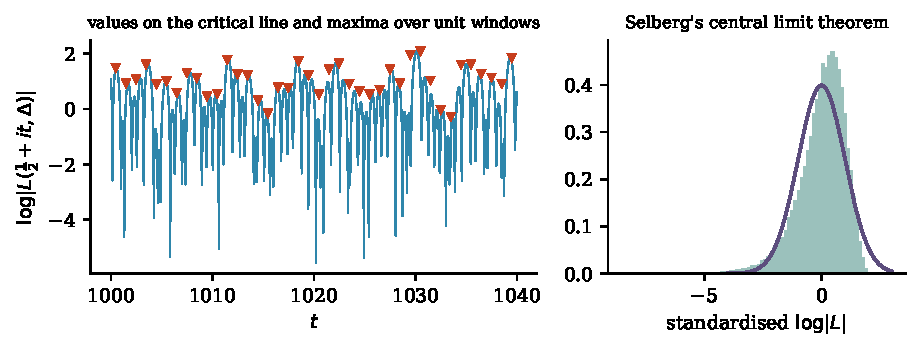
\includegraphics[width=\textwidth]{figs/selberg_clt.pdf}
\caption{Left: $\log|L(6+it,\Delta)|$ for $t\in[1000,1040]$ (the axis label uses the unitary normalisation, with centre $\frac12$), with the maximum over each unit window marked; the downward spikes are zeros. Right: histogram of the standardised values of $\log|L(6+it,\Delta)|$ at $50{,}000$ points of $[500,2500)$ against the standard normal density. The excess on the left is the exponential tail of Proposition~\ref{prop:09blefttail}.}\label{fig:09bclt}
\end{figure}

\subsection{Keating and Snaith, and the hybrid product}\label{sec:09bhybrid}

Keating and Snaith \cite{keatingsnaith2000} modelled $\zeta(\frac12+it)$ near height $T$ by the characteristic polynomial of a Haar random matrix in $\mathrm{U}(N)$ with $N=\log\frac{T}{2\pi}$, the number of zeros in a window of length $2\pi$, and computed its moments exactly.\index{Keating Snaith model}

\begin{proposition}[Keating and Snaith]\label{prop:09bks}
Let $U$ be Haar distributed in $\mathrm{U}(N)$ and $\Lambda_N=\det(I-U)=Z_N(0)$ (Section~\ref{sec:ch6ksnaith}). Then
\begin{align*}
\operatorname{Var}\log|\Lambda_N|&=\frac12\sum_{j=1}^N\psi'(j)=\frac12\Bigl(H_N+N\sum_{k>N}\frac1{k^2}\Bigr)\\
&=\frac12\bigl(\log N+\gamma_{\mathrm E}+1\bigr)+O\bigl(N^{-1}\bigr),
\end{align*}
where $\psi=\Gamma'/\Gamma$, $H_N$ is the harmonic number and $\gamma_{\mathrm E}$ is Euler's constant. For $j\ge3$ the cumulants $\kappa_j(N)$ of $\log|\Lambda_N|$ converge as $N\to\infty$ to
\[
\kappa_j(\infty)=(1-2^{1-j})(-1)^j(j-1)!\,\zeta(j-1);
\]
in particular $\kappa_3(\infty)=-\pi^2/4$ and $\kappa_4(\infty)=\frac{21}{4}\zeta(3)$.
\end{proposition}

\begin{proof}
Keating and Snaith evaluate $\E|\Lambda_N|^s=\prod_{j=1}^N\Gamma(j)\Gamma(j+s)/\Gamma(j+\frac s2)^2$ for $\operatorname{Re}s>-1$ by Selberg's integral \cite{keatingsnaith2000}. The cumulant generating function of $\log|\Lambda_N|$ is therefore
\[
K(s)=\sum_{j\le N}\bigl[\log\Gamma(j)+\log\Gamma(j+s)-2\log\Gamma(j+\tfrac s2)\bigr],
\]
and $\kappa_m=K^{(m)}(0)=(1-2^{1-m})\sum_{j\le N}\psi^{(m-1)}(j)$. For $m=2$ use $\psi'(j)=\sum_{k\ge j}k^{-2}$ and exchange the sums: $\sum_{j\le N}\psi'(j)=\sum_k\min(k,N)k^{-2}=H_N+N\sum_{k>N}k^{-2}$. Since $H_N=\log N+\gamma_{\mathrm E}+O(N^{-1})$ and $N\sum_{k>N}k^{-2}=1+O(N^{-1})$, the variance follows. For $m\ge3$ use $\psi^{(m-1)}(j)=(-1)^m(m-1)!\sum_{k\ge j}k^{-m}$; then $\sum_{j\ge1}\sum_{k\ge j}k^{-m}=\sum_kk^{1-m}=\zeta(m-1)$ converges.
\end{proof}

The random matrix model thus predicts a variance of the right growth, $\frac12\log\log T$, and also a constant, $\frac12(\gamma_{\mathrm E}+1)$. It also predicts that the higher cumulants stay bounded: the non Gaussian features of $\log|\zeta|$ at finite height should be of fixed absolute size, decaying in standard units only like powers of $\log\log T$. For our sample, with variance $1.5265$, the limits $\kappa_3(\infty)$ and $\kappa_4(\infty)$ correspond to skewness $-1.308$ and excess kurtosis $2.708$, against the observed $-1.135$ and $2.493$. The signs and sizes agree; the model is not expected to be exact here, since it ignores the arithmetic.

The arithmetic is restored by the hybrid Euler Hadamard product of Gonek, Hughes and Keating \cite{ghk2007}.\index{hybrid Euler Hadamard product} For a parameter $X\ge2$ they write $\zeta(s)=P_X(s)Z_X(s)$ up to a small error, where $P_X$ is a smoothed Euler product over the primes $p\le X$ and $Z_X$ is a smoothed Hadamard product over the zeros within about $1/\log X$ of $s$. They prove that $\E|P_X|^{2k}\sim a_k(e^{\gamma_{\mathrm E}}\log X)^{k^2}$ as $X,T\to\infty$ with $X=O((\log T)^{2-\varepsilon})$, with the arithmetic factor
\[
a_k=\prod_p\Bigl(1-\frac1p\Bigr)^{k^2}\sum_{m\ge0}\frac{d_k(p^m)^2}{p^m},
\]
conjecture that $\E|Z_X|^{2k}\sim\frac{G(k+1)^2}{G(2k+1)}\bigl(\log T/(e^{\gamma_{\mathrm E}}\log X)\bigr)^{k^2}$, the Keating Snaith moment of a matrix of size $\log T/(e^{\gamma_{\mathrm E}}\log X)$, and conjecture that the two factors are asymptotically independent, so that their moments multiply; they establish both conjectures when $k=1$ and $k=2$. The product recovers the moment conjecture $\E|\zeta|^{2k}\sim a_k\frac{G(k+1)^2}{G(2k+1)}(\log T)^{k^2}$ of Keating and Snaith and of Conrey, Farmer, Keating, Rubinstein and Snaith \cite{cfkrs2005}, and the dependence on $X$ cancels. Here $G$ is Barnes' function and $d_k$ is the $k$ fold divisor function. Reading off the coefficient of $k^2$ in the logarithm of each factor splits the variance into a prime part and a zero part. Since $\log\frac{G(k+1)^2}{G(2k+1)}=(1+\gamma_{\mathrm E})k^2+O(k^3)$ and $d_k(p^m)=k/m+O(k^2)$, the variance implied for $\zeta$ is
\begin{equation}\label{eq:09bvarzeta}
V_\zeta(T)=\frac12\Bigl(\log\log\frac{T}{2\pi}+\gamma_{\mathrm E}+1+A_\zeta\Bigr),\quad A_\zeta=\sum_p\Bigl(\log\Bigl(1-\frac1p\Bigr)+\mathrm{Li}_2\Bigl(\frac1p\Bigr)\Bigr),
\end{equation}
and we computed $A_\zeta=-0.17625$, so that the constant is $\frac12(\gamma_{\mathrm E}+1+A_\zeta)=0.70048$.

For a form of degree two the same recipe gives a conjecture we can test. Write $A_p$ for the Satake parameter of $\Delta$ at $p$, so $\tr A_p^m=2\cos m\theta_p$.

\begin{conjecture}[Variance at finite height; our formulation for $\Delta$]\label{conj:09bvar}
For $t$ uniform on $[T,2T]$,
$\operatorname{Var}\log|L(6+it,\Delta)|=V_\Delta(T)+o(1)$, where
\[
V_\Delta(T)=\frac12\Bigl(\log\Bigl(2\log\frac{T}{2\pi}\Bigr)+\gamma_{\mathrm E}+1+A_\Delta\Bigr)
\]
and
\[
A_\Delta=\sum_p\Bigl(\log\Bigl(1-\frac1p\Bigr)+\sum_{m\ge1}\frac{(2\cos m\theta_p)^2}{m^2p^m}\Bigr).
\]
\end{conjecture}

The term $\log(2\log\frac T{2\pi})$ is $\log N$ for the matrix size $N=2\log\frac{T}{2\pi}$ that matches the doubled density of zeros, and $A_\Delta$ is the coefficient of $k^2$ in the CFKRS arithmetic factor of $\Delta$, obtained exactly as for $\zeta$ from $d_k(\Delta;p^m)=k\tr A_p^m/m+O(k^2)$. The series converges by Lemma~\ref{lem:09brs}, and Exercise~\ref{ex:09bmertens} expresses $A_\Delta$ through $L(1,\Sym^2\Delta)$.

\paragraph{The arithmetic.} From $\tau(p)$ for $p\le10^5$ we find $A_\Delta=-0.898$: the partial sums are $-0.8946$, $-0.8966$, $-0.8976$ at $p\le2500$, $10^4$, $10^5$, and the identity of Exercise~\ref{ex:09bmertens} gives the limit $-0.8979$. Below we use the value $-0.8976$. At $T=1500$ the five pieces of $V_\Delta$ are
\[
\underbrace{\tfrac12\log\log T}_{0.9948}+\underbrace{\tfrac12\log2}_{0.3466}+\underbrace{\tfrac12\log\frac{\log(T/2\pi)}{\log T}}_{-0.1447}+\underbrace{\tfrac12(\gamma_{\mathrm E}+1)}_{0.7886}+\underbrace{\tfrac12A_\Delta}_{-0.4488}=1.5365 .
\]
Our sample is spread over $t\in[500,2500]$, and the average of $V_\Delta(t)$ over that range is $1.5268$, against the observed variance $1.5265$. The leading term $\frac12\log\log t$ accounts for only $65$ per cent of the observed variance. The random matrix constant without the arithmetic factor, $\frac12(\log(2\log\frac{t}{2\pi})+\gamma_{\mathrm E}+1)$, averages $1.9756$ and overshoots by $0.45$. The prime model alone, the variance of the random Euler product with the true Satake angles at the primes $p\le t$, gives $0.76$, $0.81$, $0.84$, $0.87$ at $t=500$, $1000$, $1500$, $2500$, and undershoots by about $0.7$; its deficit against $\frac12\log\log t$ comes from the negative constant $B_\Delta$ of Lemma~\ref{lem:09brs}, partly offset by the prime powers. Only the combination of Conjecture~\ref{conj:09bvar} accounts for the data, and it does so within the sampling error. The $50{,}000$ values are strongly dependent, but batch means, a moving block bootstrap and a Bartlett long run variance, with blocks or bandwidths of $1$ to $100$ units of $t$, put the standard error of the sample variance between $0.012$ and $0.018$, far below the distance of $0.45$ or more from each of the three alternatives above. Corrections of relative order $1/\log t$ are also expected. The agreement to the third decimal is therefore luck; the agreement within the sampling error, over a single range of heights, is evidence for the conjecture, not a test of its error term. The split of $V_\Delta$ into a prime part and a zero part is not unique, and the moment theorem of Gonek, Hughes and Keating concerns $X=O((\log T)^{2-\varepsilon})$, not $X=T$; what is tested is the combination $V_\Delta$, in which $X$ does not appear.

\section{A log correlated field}\label{sec:09blogcorr}

\subsection{Covariance across scales}

The variance $\frac12\log\log T$ is the sum of contributions $\frac1{2p}$ from the primes, and the dependence between nearby points is decided prime by prime. The following proposition makes this exact for the random model.\index{log correlated field}

\begin{proposition}[Covariance of the random model; this book]\label{prop:09bcov}
Let $(U_p)$ be independent and uniform on the unit circle, and for $P\ge3$ and real $h$ put $X_P(h)=\operatorname{Re}\sum_{p\le P}U_pp^{-1/2-ih}$. Then
\begin{align*}
\operatorname{Cov}\bigl(X_P(h),X_P(h')\bigr)&=\frac12\sum_{p\le P}\frac{\cos\bigl((h-h')\log p\bigr)}{p}\\
&=\frac12\log\min\Bigl(\log P,\frac{1}{|h-h'|}\Bigr)+O(1),
\end{align*}
uniformly in $P$ and in $0<|h-h'|\le1$. The same holds for the field $X^\Delta_P(h)=\operatorname{Re}\sum_{p\le P}\lambda(p)U_pp^{-1/2-ih}$, with $\lambda(p)^2/p$ in place of $1/p$ in the sum.
\end{proposition}

\begin{proof}
For independent uniform $U$, $\E\operatorname{Re}(Ua)\operatorname{Re}(Ub)=\frac12\operatorname{Re}(a\bar b)$, which gives the first identity. Put $u=|h-h'|$ and $Q=\min(P,e^{1/u})$. For $p\le Q$ we have $\cos(u\log p)=1+O(u^2\log^2p)$, and $\sum_{p\le Q}u^2\log^2p/p\ll u^2\log^2Q\le1$ by Mertens' estimate $\sum_{p\le y}\log p/p=\log y+O(1)$ and partial summation. So the primes $p\le Q$ contribute $\frac12\sum_{p\le Q}1/p+O(1)=\frac12\log\log Q+O(1)$. If $P>e^{1/u}$ the remaining primes contribute $\frac12\sum_{e^{1/u}<p\le P}\cos(u\log p)/p$. By the prime number theorem with remainder $O(y/\log^2y)$ and partial summation, this equals $\frac12\int_{1/u}^{\log P}\cos(uv)\,\frac{dv}{v}+O(u)$, and the integral is $\int_1^{u\log P}\cos w\,\frac{dw}{w}$, which is bounded uniformly. Since $\log\log Q=\log\min(\log P,1/u)$, the formula follows. For $X^\Delta_P$ the same argument applies with Lemma~\ref{lem:09brs} and the prime number theorem for $L(s,\Delta\times\Delta)=\zeta(s)L(s,\Sym^2\Delta)$ in the form $\sum_{p\le y}\lambda(p)^2\log p=y+O(y/\log^2y)$, which follows from the zero free regions used in the proof of the lemma, in place of Mertens and the prime number theorem.
\end{proof}

At $h=h'$ the variance is $\frac12\log\log P+O(1)$. Two points at distance $u$ are almost perfectly correlated in the primes up to $e^{1/u}$ and almost uncorrelated beyond, so for $1/\log P\le u\le1$ the correlation coefficient is $\log(1/u)/\log\log P+O(1/\log\log P)$. This is the defining property of a log correlated field. For $\zeta$ itself the analogous statement is a theorem of Bourgade \cite{bourgade2010}: for shifts $h_1,\dots,h_k$ with $|h_i-h_j|=(\log T)^{-c_{ij}+o(1)}$, $0\le c_{ij}\le1$, the vector $(\log\zeta(\frac12+i(t+h_j)))_j/\sqrt{\frac12\log\log T}$ is asymptotically complex Gaussian, with correlation $c_{ij}$ between the real parts. Thus, to leading order, the covariance of $\log|\zeta|$ at distance $u$ is $\frac12\log(1/u)$ for $1/\log T\le u\le1$, saturating at $\frac12\log\log T$ below the scale $1/\log T$ of the zero spacings.

\subsection{The branching picture}

Group the primes into blocks $e^{e^{k-1}}<p\le e^{e^k}$, $k=1,\dots,n$ with $n=\log\log T$, and write the field of Proposition~\ref{prop:09bcov} with $P=T$ as $X_T(h)=\sum_kY_k(h)$, with $Y_k$ the contribution of block $k$. Each block has variance about $\frac12$, since $\sum1/p$ over a block is about $1$. Inside a window $|h|\le1$, $Y_k$ is essentially constant on intervals of length $e^{-k}$ and essentially independent across such intervals, because its frequencies $\log p$ are about $e^k$. So $X_T$ restricted to the window is approximately a branching random walk: a tree in which every vertex at level $k$ has about $e$ children, each level adds an independent Gaussian increment of variance $\frac12$, and the leaves at level $n$ are the effectively distinct values of the field, about $e^n=\log T$ per unit length, one for each interval of length $1/\log T$, the scale of the zero spacings.\index{branching random walk} Figure~\ref{fig:09bfield} shows the picture for the field
\[
R_X(t)=\sum_{p\le X}\frac{2\cos\theta_p\cos(t\log p)}{\sqrt p}=\operatorname{Re}\sum_{p\le X}2\cos\theta_p\,p^{-1/2-it},
\]
the prime part of $\log|L_{\mathrm{rand}}(\frac12+it)|$ for the Sato Tate random Euler product of Chapter~\ref{ch:09}, with $\theta_p$ independent with the Sato Tate law, built up through the levels $X=e^{e^{k/2}}$, $k=1,\dots,5$ (that is $5.2$, $15.2$, $88.4$, $1618$, $195339$), and then $X=10^6$.

\begin{figure}[t]\centering
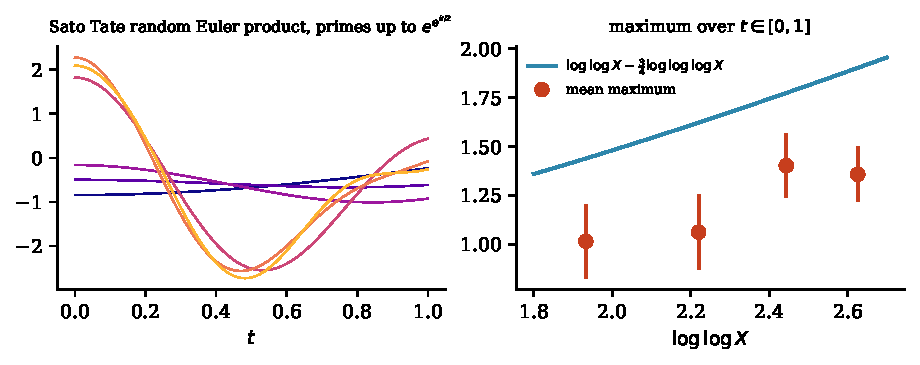
\includegraphics[width=\textwidth]{figs/random_field.pdf}
\caption{Left: one realisation of the field $R_X(t)=\sum_{p\le X}2\cos\theta_p\cos(t\log p)/\sqrt p$ of the Sato Tate random Euler product on $t\in[0,1]$, built up by adding the primes in successive ranges $p\le e^{e^{k/2}}$, $k=1,\dots,5$, and then $p\le10^6$; each level refines the previous one on a finer scale, which is the branching structure. Right: mean of $\max_{t\in[0,1]}R_X(t)$ for $X=10^3,10^4,10^5,10^6$ ($300$, $200$, $80$ and $30$ draws) against the curve $\log\log X-\frac34\log\log\log X$. The error bars are one standard deviation divided by $\sqrt{30}$ at every point, which overstates the standard error of the first three means. The offset is an additive constant that the theory does not determine.}\label{fig:09bfield}
\end{figure}

The maximum of a branching random walk is understood in detail, and it is the source of the constant $\frac34$. We isolate the computation in a continuous model where it can be done exactly. Let $b\ge2$ be an integer, $\sigma>0$, and let $\{B_v(s):0\le s\le n\}$, indexed by the $b^n$ leaves $v$ of the $b$ ary tree of depth $n$, be Brownian motion indexed by the tree: each edge carries an independent Brownian path of duration one and variance $\sigma^2$ per unit time, and $B_v$ is the concatenation along the path from the root to $v$. At integer times this is a branching random walk with $N(0,\sigma^2)$ increments. Put
\[
c=\sigma\sqrt{2\log b},\qquad\theta=\frac{c}{\sigma^2}=\frac{\sqrt{2\log b}}{\sigma},\qquad x_n=cn-a\log n
\]
for a constant $a>0$.

\begin{proposition}[First moments with and without the ballot constraint; this book]\label{prop:09bballot}
Fix $y\ge0$. Let $N_n(y)$ be the number of leaves with $B_v(n)\ge x_n+y$, and $Z_n(y)$ the number of leaves with $B_v(n)\in[x_n+y,x_n+y+1]$ and $B_v(s)\le\frac snx_n+y+1$ for all $s\in[0,n]$. As $n\to\infty$,
\[
\E N_n(y)\sim\frac{\sigma}{c\sqrt{2\pi}}\,n^{\theta a-\frac12}e^{-\theta y},\qquad
\E Z_n(y)\sim\kappa\,(1+y)\,n^{\theta a-\frac32}e^{-\theta y},
\]
with $\kappa=2(\theta-1+e^{-\theta})/(\sigma^3\theta^2\sqrt{2\pi})$.
In particular the choice $a=\frac1{2\theta}$ makes $\E N_n$ of order one, while $a=\frac3{2\theta}$ makes $\E Z_n(y)\to\kappa(1+y)e^{-\theta y}$, and for that choice $\E N_n(y)$ grows like $n$.
\end{proposition}

\begin{proof}
Each $B_v(n)$ is $N(0,\sigma^2n)$ with density $\varphi_n$. For $z=x_n+y+u$ with $u$ bounded,
\begin{align*}
\frac{z^2}{2\sigma^2n}&=\frac{c^2n}{2\sigma^2}-\frac{c}{\sigma^2}(a\log n-y-u)+O\Bigl(\frac{\log^2n}{n}\Bigr)\\
&=n\log b-\theta a\log n+\theta(y+u)+o(1),
\end{align*}
so $b^n\varphi_n(z)=(\sigma\sqrt{2\pi n})^{-1}n^{\theta a}e^{-\theta(y+u)}(1+o(1))$. The first claim follows from $\E N_n(y)=b^n\Prob(B(n)\ge x_n+y)$ and the Mills ratio $\Prob(B(n)\ge z)\sim\sigma^2n\,\varphi_n(z)/z$ with $z\sim cn$. For the second, condition on $B_v(n)=x_n+y+u$, $u\in[0,1]$. The process $R(s)=B_v(s)-\frac snx_n$ is then a Brownian bridge of variance $\sigma^2$ per unit time from $0$ to $y+u$ on $[0,n]$, and the constraint is $R\le y+1$. By the reflection principle a bridge from $0$ to $e$ of duration $n$ stays below a level $h>\max(0,e)$ with probability $1-\exp(-2h(h-e)/(\sigma^2n))$. With $h=y+1$ and $e=y+u$ this is $\frac{2(1+y)(1-u)}{\sigma^2n}(1+o(1))$. Integrating against $b^n\varphi_n(x_n+y+u)\,du$ over $[0,1]$ gives
\[
\E Z_n(y)\sim\frac{2(1+y)}{\sigma^3\sqrt{2\pi}}\,n^{\theta a-\frac32}e^{-\theta y}\int_0^1(1-u)e^{-\theta u}\,du,
\]
and $\int_0^1(1-u)e^{-\theta u}du=(\theta-1+e^{-\theta})/\theta^2$.
\end{proof}

The proposition explains the two corrections. The naive first moment places the maximum at $cn-\frac1{2\theta}\log n$. But the leaves that reach that height are overwhelmingly descendants of ancestors that were already too high at intermediate levels, and such ancestors are rare; they occur with probability tending to zero, while each of them produces a large number of high leaves, which is how the expectation can be large while the typical count is zero. Requiring the path to stay below the straight line to its endpoint, a ballot constraint, costs a factor $1/n$, and this moves the correct centring to $m_n=cn-\frac{3}{2\theta}\log n$. The factor $1+y$ is the ballot probability for a path that starts at distance $y+1$ below the barrier, and it produces a right tail of the form $ye^{-\theta y}$ for the maximum. That the constrained first moment gives the right answer is the content of the following theorem.

\begin{theorem}[Bramson; Addario Berry and Reed; A\"id\'ekon]\label{thm:09bbrw}
For the branching random walk above, with $M_n=\max_vB_v(n)$ and $m_n=cn-\frac{3}{2\theta}\log n$, the sequence $M_n-m_n$ is tight, and it converges in law: there are a constant $C^*>0$ and a positive random variable $D_\infty$, the limit of the derivative martingale, such that
\[
\Prob(M_n\le m_n+y)\longrightarrow\E\bigl[\exp\bigl(-C^*D_\infty e^{-\theta y}\bigr)\bigr]\qquad(y\in\R).
\]
\end{theorem}

The limit is a Gumbel law randomly shifted by $\theta^{-1}\log(C^*D_\infty)$. Bramson \cite{bramson1978} proved the $\frac{3}{2\theta}\log n$ correction for branching Brownian motion, where Lalley and Sellke \cite{lalleysellke1987} identified the derivative martingale; Addario Berry and Reed \cite{addarioberryreed2009} proved tightness for branching random walks, and A\"id\'ekon \cite{aidekon2013} the convergence in law. The book of Bovier \cite{bovier2017} and the lecture notes of Kistler \cite{kistler2015} explain the method, whose heart is a refinement of Proposition~\ref{prop:09bballot}.

For the zeta field the parameters are fixed by the variance and the number of leaves. Take $b=2$ and $n_2=\lfloor\log\log T/\log2\rfloor$ levels of variance $\sigma^2=\frac12\log2$, so that a leaf has variance $\frac12\log\log T$ and there are $2^{n_2}\approx\log T$ leaves. Then $c=\log2$ and $\theta=2$, so $cn_2=\log\log T+O(1)$, $\frac3{2\theta}\log n_2=\frac34\log\log\log T+O(1)$, and the right tail is $ye^{-2y}$. The value $\theta=2$ does not depend on the choice of tree: per unit of $\log\log T$ the field gains variance $\frac12$ while the number of leaves is multiplied by $e$, so the speed is $c=1$ per unit and $\theta=c/\sigma^2=2$.

\subsection{The Fyodorov Hiary Keating conjecture}

\begin{conjecture}[Fyodorov, Hiary and Keating \cite{fhk2012,fyodorovkeating2014}]\label{conj:09bfhk}\index{Fyodorov Hiary Keating conjecture}
Let $\tau$ be uniform on $[T,2T]$. Then
\[
\max_{|h|\le1}\log\bigl|\zeta\bigl(\tfrac12+i(\tau+h)\bigr)\bigr|=\log\log T-\tfrac34\log\log\log T+\mathcal{M}_T,
\]
where $\mathcal{M}_T$ converges in law to a random variable $\mathcal{M}$ with $\Prob(\mathcal{M}>y)\sim Cye^{-2y}$ as $y\to\infty$.
\end{conjecture}

Fyodorov, Hiary and Keating reached the conjecture through random matrix theory, predicting by a freezing transition that $\max_\phi\log|\det(I-Ue^{-i\phi})|=\log N-\frac34\log\log N+O(1)$ for Haar unitary $U$, and matching $N=\log T$. For the matrices they also predicted the law of the bounded term, and they compared their predictions with Hiary's computations of $\zeta$ at large height. The tail $ye^{-2y}$ is expected to carry over to $\zeta$, but the law itself is not expected to coincide with the random matrix one \cite{fyodorovkeating2014,abr2023}. The branching random walk gives the same centring.

What is proved is the following.

\begin{theorem}\label{thm:09bfhkproved}
Let $\tau$ be uniform on $[T,2T]$, and write
\[
M_T=\max_{|h|\le1}\log\bigl|\zeta\bigl(\tfrac12+i(\tau+h)\bigr)\bigr|,\qquad m_T=\log\log T-\tfrac34\log\log\log T .
\]
\begin{enumerate}
\item (First order.) For every $\varepsilon>0$, with probability tending to one, $|M_T-\log\log T|\le\varepsilon\log\log T$. This is due to Najnudel \cite{najnudel2018}, assuming the Riemann hypothesis, and to Arguin, Belius, Bourgade, Radziwi\l\l\ and Soundararajan \cite{abbrs2019} unconditionally.
\item (Upper tail.) Arguin, Bourgade and Radziwi\l\l\ \cite{abr2020} prove that $\Prob(M_T>m_T+y)\ll ye^{-2y}$ for all large $T$, uniformly in $y\ge1$; in particular $M_T-m_T$ is bounded above in probability.
\item (Lower bounds.) In a second paper \cite{abr2023} the same authors prove that $\Prob(M_T<m_T-y)\to0$ as $y\to\infty$, uniformly in large $T$, and that $\Prob(M_T>m_T+y)\gg ye^{-2y}$ for $10\le y\le\sqrt{\log\log T}$. Together the two papers show that $M_T-m_T$ is tight, with right tail of exact order $ye^{-2y}$ in that range.
\end{enumerate}
\end{theorem}

Before the work of Arguin, Bourgade and Radziwi\l\l, Harper \cite{harper2019} proved that with probability tending to one
\[
\max_{|h|\le1/2}\log\bigl|\zeta\bigl(\tfrac12+i(\tau+h)\bigr)\bigr|\le\log\log T-\bigl(\tfrac34+o(1)\bigr)\log\log\log T,
\]
the first upper bound with the correct second term, by bounding the critical partition function $\int_{|h|\le1/2}|\zeta(\frac12+i(\tau+h))|^2dh$. What remains open is the convergence in law of $\mathcal{M}_T$ (tightness gives only subsequential limits), the tail constant $C$, and the form of the limit, which by analogy with Theorem~\ref{thm:09bbrw} and with the random matrix case one expects to be a randomly shifted Gumbel law. For random unitary matrices more is known: the leading order is due to Arguin, Belius and Bourgade \cite{abb2017}, the second order term $-\frac34\log\log N$ to Paquette and Zeitouni \cite{paquettezeitouni2018}, tightness at the scale $\log N-\frac34\log\log N$ to Chhaibi, Madaule and Najnudel \cite{cmn2018}, and Paquette and Zeitouni \cite{paquettezeitouni2022} proved, for the circular $\beta$ ensembles, convergence in law to the sum of a Gumbel variable and an independent variable defined through a derivative martingale.

For a degree two form the Rankin Selberg variance and the doubled density of zeros change only $O(1)$ terms in the heuristic: the leaves are the $2\log T$ effectively distinct values per unit window, and $\log\log(T^2)=\log\log T+\log2$. We therefore expect $\max_{|h|\le1}\log|L(6+i(\tau+h),\Delta)|=\log\log T-\frac34\log\log\log T+O_{\Prob}(1)$, with an additive constant that differs from that of $\zeta$. We are not aware of a proof for $\Delta$, even to first order, though we expect the methods of \cite{abbrs2019} to extend.

\paragraph{Data.} We split $[500,2500]$ into $2000$ unit windows and recorded the maximum of $\log|L(6+it,\Delta)|$ in each (Figure~\ref{fig:09bclt}, left). The mean of the window maxima is $1.1010$ with standard deviation $0.5674$, and the mean of $\log\log t-\frac34\log\log\log t$ at the window centres is $1.4655$. The difference has mean $-0.3645$ and standard deviation $0.5657$, so the standard error of the mean difference is about $0.013$ (the windows are adjacent, so slightly more in truth). This is consistent with a bounded additive correction, which neither the conjecture nor the theorem determines. It is not evidence for the $\frac34$: over $[500,2500]$ the term $\frac34\log\log\log t$ varies only between $0.45$ and $0.54$, so it cannot be separated from an unknown constant. For the field $R_X$ of Figure~\ref{fig:09bfield} the mean maxima over $t\in[0,1]$ are $1.015$, $1.062$, $1.402$, $1.358$ for $X=10^3,10^4,10^5,10^6$, from $300$, $200$, $80$ and $30$ draws with standard deviations $1.03$, $1.05$, $0.89$, $0.77$, against $\log\log X-\frac34\log\log\log X=1.438$, $1.622$, $1.773$, $1.902$. The differences, $-0.42$, $-0.56$, $-0.37$, $-0.54$, with standard errors $0.06$, $0.07$, $0.10$, $0.14$, are consistent with a constant offset (weighted mean $-0.47$, $\chi^2=3.3$ on $3$ degrees of freedom), and the decrease of the mean maximum from $10^5$ to $10^6$ is within noise; the range of $X$ is too short to separate the $\frac34\log\log\log X$ term from the constant. The model is also not stationary: $\E R_X(t)^2=\frac12\sum_{p\le X}(1+\cos(2t\log p))/p$ is close to $\log\log X$ rather than $\frac12\log\log X$ near $t=0$, so we use it only to show the branching mechanism.

\section{Multiplicative chaos}\label{sec:09bchaos}

Exponentiating a log correlated field produces a random measure. Let $Y$ be a centred Gaussian field on an interval with $\E Y(x)Y(x')=\log\frac{1}{|x-x'|}+g(x,x')$, $g$ bounded and continuous. The field is not defined pointwise, but its regularisations $Y_\varepsilon$ at scale $\varepsilon$ are, and Kahane \cite{kahane1985} showed that, for suitable regularisations and $0<\gamma<\sqrt2$, the measures
\[
M_{\gamma,\varepsilon}(dx)=e^{\gamma Y_\varepsilon(x)-\frac{\gamma^2}2\E Y_\varepsilon(x)^2}\,dx
\]
converge, as $\varepsilon\to0$, to a nontrivial random measure $M_\gamma$, the \emph{Gaussian multiplicative chaos}\index{multiplicative chaos} of parameter $\gamma$; later work showed that the limit does not depend on the regularisation \cite{rhodesvargas2014}, and it is carried by a set of points where $Y$ is atypically large, of dimension $1-\gamma^2/2$. For $\gamma\ge\sqrt2$ the normalised measures tend to zero. At the critical value $\gamma=\sqrt2$ a nontrivial limit is obtained either from the derivative martingale or by the Seneta Heyde normalisation $\sqrt{\log(1/\varepsilon)}\,M_{\sqrt2,\varepsilon}$, and the two constructions agree up to a constant factor, as shown by Duplantier, Rhodes, Sheffield and Vargas \cite{dsrv2014,dsrv2014b}. The survey of Rhodes and Vargas \cite{rhodesvargas2014} gives the theory.

The dictionary with $\zeta$ follows from Proposition~\ref{prop:09bcov}. The field $\log|\zeta(\frac12+i(\tau+x))|$ has covariance $\frac12\log\frac1{|x-x'|}$ down to the scale $\varepsilon=1/\log T$, so $Y=\sqrt2\log|\zeta|$ is normalised as above, and
\[
|\zeta|^{2\beta}=e^{2\beta\log|\zeta|}=e^{\sqrt2\beta Y}:\qquad\gamma=\sqrt2\,\beta .
\]
The measures $|\zeta(\frac12+i(\tau+x))|^{2\beta}dx$, normalised by their mean $(\log T)^{\beta^2}$ up to constants, are therefore expected to converge to subcritical chaos for $\beta<1$, and $\beta=1$, the measure $|\zeta|^2dx$ whose mean is the classical Hardy Littlewood second moment, is exactly critical. The critical measure carries the information about the maximum. Its Seneta Heyde factor $\sqrt{\log\log T}$ is the inverse of the probability, of order $1/\sqrt n$ with $n=\log\log T$ levels, that a random walk stays below a barrier; Proposition~\ref{prop:09bballot} computes the same constraint for a bridge, whose cost is $1/n$.

Saksman and Webb proved a statement of this kind for $\zeta$ itself rather than for powers of its modulus.

\begin{theorem}[Saksman and Webb \cite{saksmanwebb2020}]\label{thm:09bsw}
Let $\omega$ be uniform on $[0,1]$. As $T\to\infty$, the random generalised function $x\mapsto\zeta(\frac12+ix+i\omega T)$ on a fixed bounded interval converges in law, in the Sobolev space $W^{-\alpha,2}$ for any $\alpha>\frac12$, to the random generalised function
\[
\zeta_{\mathrm{rand}}(\tfrac12+ix)=\lim_{N\to\infty}\prod_{p\le N}\bigl(1-U_pp^{-1/2-ix}\bigr)^{-1},
\]
with $(U_p)$ independent and uniform on the unit circle, the limit taken in the same space. Moreover $\zeta_{\mathrm{rand}}(\frac12+ix)$ is the product of a random smooth function and a complex Gaussian multiplicative chaos, the exponential of a complex Gaussian field whose real and imaginary parts are log correlated.
\end{theorem}

No normalisation is needed: the shifted zeta function itself has a limit, but only as a generalised function. The chaos is complex: the exponent $\sum_pU_pp^{-1/2-ix}$ has real and imaginary parts, each with covariance $\frac12\log\frac1{|x-x'|}+O(1)$. Saksman and Webb formulate the convergence of $|\zeta|^{2\beta}dx$ to subcritical chaos for $\beta<1$ as a conjecture, together with the critical case: that
\[
\sqrt{\log\log T}\,(\log T)^{-1}\bigl|\zeta\bigl(\tfrac12+ix+i\omega T\bigr)\bigr|^2dx
\]
converges in law to a constant multiple of a critical chaos measure. Both conjectures are open in print as we write; Gorodetsky and Wong \cite{gorodetskywong2025} report that the critical one will be established in forthcoming work of Harper, Saksman and Webb. For the truncated random Euler product the analogous critical statement is a theorem of Saksman and Webb.

Figure~\ref{fig:09bchaos} shows, for a single realisation, the squared modulus of the random Euler product $\prod_{p\le N}(1-U_pp^{-1/2-it})^{-1}$ truncated at $N=2\times10^5$, on a logarithmic scale. The measure is concentrated in thin spikes separated by long stretches where it is small. This is the behaviour expected near criticality: for $\gamma<\sqrt2$ the chaos is carried by a set of dimension $1-\gamma^2/2$, which shrinks to dimension zero at the critical value.

\begin{figure}[t]\centering
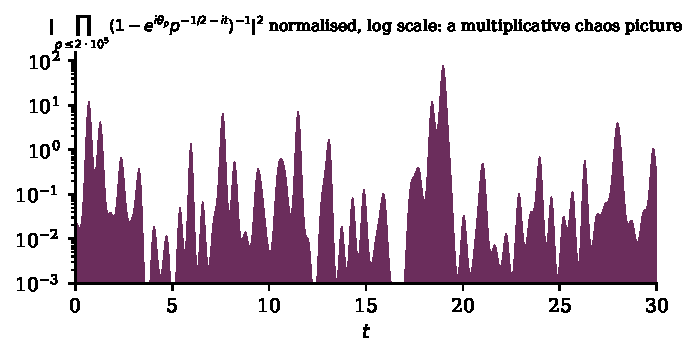
\includegraphics[width=\textwidth]{figs/chaos.pdf}
\caption{One realisation of $|\prod_{p\le2\cdot10^5}(1-U_pp^{-1/2-it})^{-1}|^2$ for $t\in[0,30]$, with $U_p$ independent and uniform on the unit circle (the Steinhaus random Euler product), divided by its mean over the window, on a logarithmic scale. The mass sits on a sparse set of spikes: a picture of critical multiplicative chaos ($\beta=1$, $\gamma=\sqrt2$), cut off at the scale $1/\log(2\cdot10^5)$.}\label{fig:09bchaos}
\end{figure}

\paragraph{Moments of moments.} The freezing transition behind Conjecture~\ref{conj:09bfhk} is visible in the moments of the chaos. For $U$ Haar in $\mathrm{U}(N)$ and $Z_N(\phi)=\det(I-Ue^{-i\phi})$, Fyodorov and Keating \cite{fyodorovkeating2014} studied
\[
\mathrm{MoM}_N(k,\beta)=\E\Bigl[\Bigl(\frac1{2\pi}\int_0^{2\pi}|Z_N(\phi)|^{2\beta}d\phi\Bigr)^k\Bigr]
\]
and conjectured that it grows like $N^{k\beta^2}$ when $k\beta^2<1$ and like $N^{k^2\beta^2-k+1}$ when $k\beta^2>1$. Below the transition the $k$th moment of the total mass of the limiting chaos is finite, and $\mathrm{MoM}_N$ is of the order of the $k$th power of the mean; above it, the moment is dominated by the neighbourhood of the maximum. Bailey and Keating \cite{baileykeating2019} proved that for positive integers $k$ and $\beta$, $\mathrm{MoM}_N(k,\beta)$ is a polynomial in $N$ of degree $k^2\beta^2-k+1$, confirming the exponent in the second regime for integer parameters. Relatedly, Arguin, Belius and Bourgade \cite{abb2017} proved that the free energy $\frac1{\log N}\log\frac1{2\pi}\int_0^{2\pi}|Z_N(\phi)|^{2\beta}d\phi$ converges in probability to $\beta^2$ for $\beta\le1$ and to $2\beta-1$ for $\beta\ge1$, the slope $2$ above the transition reflecting a maximum of $\log|Z_N|$ equal to $\log N$ to first order.

\section{Random multiplicative functions}\label{sec:09bharper}

The random Euler product has a Dirichlet series, and its coefficients are a random multiplicative function. In the \emph{Steinhaus model} $f(p)=U_p$ are independent and uniform on the unit circle and $f$ is completely multiplicative; in the \emph{Rademacher model} of Wintner \cite{wintner1944} $f(p)=\pm1$ with independent fair signs and $f$ is supported on squarefree integers. Write $S(x)=\sum_{n\le x}f(n)$.\index{random multiplicative function}

For the Steinhaus model $\E f(n)\overline{f(m)}=\mathbb{I}_{n=m}$ by unique factorisation, so $\E|S(x)|^2=\lfloor x\rfloor$. If $S(x)/\sqrt x$ were approximately a standard complex Gaussian, we would have $\E|S(x)|\sim\frac{\sqrt\pi}{2}\sqrt x=0.886\sqrt x$. Helson \cite{helson2010} conjectured instead that $\E|S(x)|=o(\sqrt x)$, and Harper proved it with the exact rate.

\begin{theorem}[Harper \cite{harper2020}]\label{thm:09bharper}\index{Harper's theorem}
Let $f$ be a Steinhaus random multiplicative function. Uniformly for all large $x$ and $0\le q\le1$,
\[
\E|S(x)|^{2q}\asymp\Bigl(\frac{x}{1+(1-q)\sqrt{\log\log x}}\Bigr)^q .
\]
In particular $\E|S(x)|$ is of exact order $\sqrt x\,(\log\log x)^{-1/4}$. The same bounds hold for the Rademacher model.
\end{theorem}

Harper calls this better than square root cancellation. The mechanism is critical multiplicative chaos, and it can be seen through an exact identity.

\begin{lemma}[Plancherel identity]\label{lem:09bplancherel}
Let $f$ be any function on the positive integers with $|f|\le1$, $S(u)=\sum_{n\le u}f(n)$ and $F(s)=\sum_nf(n)n^{-s}$. For $\sigma>1$,
\[
\int_1^\infty\frac{|S(u)|^2}{u^{1+2\sigma}}\,du=\frac{1}{2\pi}\int_{-\infty}^\infty\frac{|F(\sigma+it)|^2}{|\sigma+it|^2}\,dt .
\]
\end{lemma}

\begin{proof}
By partial summation $F(s)=s\int_1^\infty S(u)u^{-s-1}du$ for $\operatorname{Re}s>1$. Put $g(v)=S(e^v)e^{-\sigma v}$ for $v\ge0$ and $g=0$ for $v<0$; then $g\in L^1\cap L^2$ since $|S(u)|\le u$ and $\sigma>1$, and its Fourier transform is $\int_0^\infty S(e^v)e^{-(\sigma+it)v}dv=F(\sigma+it)/(\sigma+it)$. Plancherel's theorem and the substitution $u=e^v$ give the identity.
\end{proof}

For the Steinhaus model the identity continues to hold almost surely for $\sigma>\frac12$, by the same argument once one knows that $S(u)\ll u^{1/2+\varepsilon}$ almost surely, which follows from the method Wintner used for the Rademacher model. Harper works at $\sigma=\frac12+1/\log x$, where the left side is a weighted average of $|S(u)|^2/u$ over $u$ up to about $x$, on a logarithmic scale, and the right side is, up to the factor $\frac1{2\pi}$, the total mass of the measure $|F(\frac12+\frac1{\log x}+it)|^2dt/|\frac12+it|^2$. Since $\log|F(\frac12+\frac1{\log x}+it)|$ is approximately the log correlated field of Proposition~\ref{prop:09bcov} with $P=x$, this is a critical chaos measure, cut off at scale $1/\log x$. Its expectation is of order $\log x$, but its typical size is of order $\log x/\sqrt{\log\log x}$, the Seneta Heyde factor again. Conditionally on the values $f(p)$ for the small primes, $S(x)$ is roughly Gaussian with variance of the order of $\frac{x}{\log x}$ times the total mass, so that
\[
\E|S(x)|\approx\sqrt{\frac{x}{\log x}}\cdot\sqrt{\frac{\log x}{\sqrt{\log\log x}}}=\frac{\sqrt x}{(\log\log x)^{1/4}} .
\]
Harper's proof turns each step of this heuristic into an inequality, and the hard step is the upper bound for low moments of the critical chaos mass, which he proves with a barrier argument of ballot type for the random walk formed by the logarithms of the partial Euler products.

\paragraph{Data.} We drew $400$ Steinhaus functions and computed $S(x)$ for $x\le10^6$. The estimates of $\E|S(x)|/\sqrt x$ at $x=10^3,3\cdot10^3,10^4,3\cdot10^4,10^5,3\cdot10^5,10^6$ are $0.773$, $0.765$, $0.807$, $0.798$, $0.778$, $0.777$, $0.781$, and their ratios to $(\log\log x)^{-1/4}$ are $0.91$, $0.92$, $0.98$, $0.99$, $0.97$, $0.98$, $0.99$ (Figure~\ref{fig:09bharper}). Since $\E|S(x)|^2=\lfloor x\rfloor$, the standard deviation of $|S(x)|/\sqrt x$ is about $\sqrt{1-0.78^2}\approx0.63$, so each estimate has a standard error of about $0.03$; the estimates at different $x$ come from the same $400$ functions and are correlated. Every estimate lies between two and a half and four standard errors below the Gaussian value $0.886$, which is the qualitative content of the theorem. The rate is another matter: over this range $(\log\log x)^{-1/4}$ falls only from $0.848$ to $0.786$, about two standard errors, and the estimates do not decrease monotonically, so the data are consistent with the theorem but cannot confirm the exponent $\frac14$. Gorodetsky and Wong \cite{gorodetskywong2025} have since proved that $(\log\log x)^{1/4}S(x)/\sqrt x$ converges in distribution, answering a question of Harper; since Theorem~\ref{thm:09bharper} with $q=\frac34$ makes these variables uniformly integrable, $c(x)=\E|S(x)|(\log\log x)^{1/4}/\sqrt x$ converges too. We know of no closed form for the limit, and our ratios are only rough estimates of it (Computational Problem~\ref{cp:09bharper}).

\begin{figure}[t]\centering
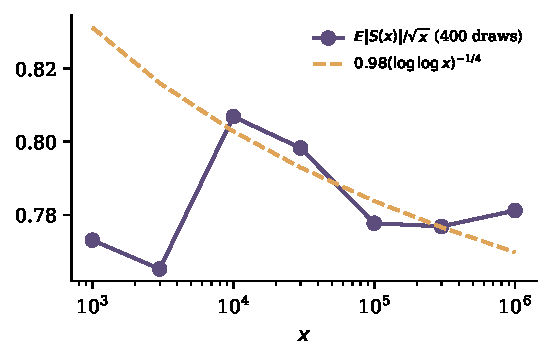
\includegraphics[width=0.62\textwidth]{figs/harper.pdf}
\caption{Estimates of $\E|S(x)|/\sqrt x$ for the Steinhaus random multiplicative function from $400$ draws (standard error about $0.03$ per point), against $0.98(\log\log x)^{-1/4}$: the rate of Theorem~\ref{thm:09bharper}, with the constant $0.98$ chosen to match the data, since the theorem gives none. A complex Gaussian with the same second moment would give $0.886$.}\label{fig:09bharper}
\end{figure}

\paragraph{Deterministic consequences.} Harper transferred the mechanism to deterministic families. For a large prime $r$ and Dirichlet characters $\chi$ modulo $r$, the sums $\sum_{n\le x}\chi(n)$ have mean square $x$ over $\chi$ when $x<r$, by orthogonality; Harper \cite{harper2023} showed that their first absolute moment is $O(\sqrt x/(\log\log(10L))^{1/4})$ with $L=\min(x,r/x)$, hence $o(\sqrt x)$ whenever $x\to\infty$ and $r/x\to\infty$, and proved the analogous statement for zeta sums $\sum_{n\le x}n^{it}$ with $t$ uniform on $[0,T]$ and $L=\min(x,T/x)$. Averaging over characters makes the $\chi(p)$ behave like the Steinhaus $f(p)$ to the extent needed. Sharp bounds for higher moments of random multiplicative functions, where Gaussian heuristics fail in the opposite direction, are in the companion paper of Harper \cite{harper2019b}.

\section{Pair correlation of the zeros of $L(s,\Delta)$}\label{sec:09bpair}

Up to a smooth term, $\log|L|$ is the logarithmic potential of the zeros, so its log correlated structure and its constants, such as the $\frac12(\gamma_{\mathrm E}+1)$ of Proposition~\ref{prop:09bks}, record how rigidly the zeros are spaced. We now look at the zeros directly.

Montgomery's theorem was stated in Chapter~\ref{ch:06} (Theorem~\ref{thm:ch6mont}): assuming the Riemann hypothesis, the pair correlation of the normalised zeros of $\zeta$ agrees with $1-(\sin\pi u/\pi u)^2$ for test functions whose Fourier transform is supported in $(-1,1)$ \cite{montgomery1973}. The pair correlation conjecture asserts the same for all test functions; the stronger GUE conjecture asserts that all $n$ level correlations, and with them all local statistics such as the nearest neighbour spacing law, are those of the Gaussian unitary ensemble.\index{pair correlation}

\begin{theorem}[Rudnick and Sarnak \cite{rudnicksarnak1996}]\label{thm:09brs}
Let $\pi$ be a cuspidal automorphic representation of $\GL_m(\A_\Q)$, assume the Riemann hypothesis for $L(s,\pi)$, and for $m\ge4$ assume their Hypothesis H on the coefficients at prime powers (it has since been proved for $m=4$, so it is needed only for $m\ge5$). Let the ordinates of the zeros be normalised to have mean spacing one. Then for each $n\ge2$ the $n$ level correlations of the normalised ordinates agree with those of the Gaussian unitary ensemble, for test functions whose Fourier transform is supported in $\sum_j|\xi_j|<2/m$.
\end{theorem}

For $n=2$ and a translation invariant test function the support condition reads $|\alpha|<1/m$, so for $\zeta$ ($m=1$) it is Montgomery's range and for $L(s,\Delta)$ ($m=2$) it is $|\alpha|<\frac12$. Within its range, the theorem shows that the local statistics of zeros at large height are universal: they do not see the degree, the level or the Sato Tate group, in contrast with the low lying zeros of families of Chapter~\ref{ch:06}. For $\Delta$ we normalise by the smooth counting function: with $\vartheta$ the phase of the Hardy function $Z_\Delta$ of the Conventions,
\[
\vartheta(t)=\operatorname{Im}\log\Gamma(6+it)-t\log2\pi=t\log\frac{t}{2\pi e}+\frac{11\pi}{4}+O\Bigl(\frac1t\Bigr),
\]
the number of zeros with ordinates in $(T_1,T_2]$ is $(\vartheta(T_2)-\vartheta(T_1))/\pi+O(\log T_2)$, and the unfolded ordinates are $\tilde\gamma=\vartheta(\gamma)/\pi$.

The nearest neighbour spacing law of the Gaussian unitary ensemble is Gaudin's \cite{gaudin1961}: $p_2(s)=\frac{d^2}{ds^2}\det(I-K_s)$, where $K_s$ is the sine kernel $\frac{\sin\pi(x-y)}{\pi(x-y)}$ acting on $L^2[0,s]$; its variance is about $0.180$ \cite{mehta2004}. The Wigner surmise $p_W(s)=\frac{32}{\pi^2}s^2e^{-4s^2/\pi}$, the exact law for $2\times2$ matrices, is a close approximation with variance $\frac{3\pi}8-1=0.178$.

\paragraph{Data.} We located the zeros of $L(s,\Delta)$ with ordinates in $[500,2000]$ as sign changes of $Z_\Delta$ on a grid of step $0.04$, computed with PARI/GP. There are $2495$ of them, against $(\vartheta(2000)-\vartheta(500))/\pi=2494.8$. Sign changes miss any pair of zeros that falls in one grid cell, so we repeated the search on a grid of step $0.01$: it finds the same $2495$ zeros, with smallest spacing $0.122$ in normalised units. Under the Gaudin law, with density about $\frac{\pi^2}3s^2$ near $0$, the expected number of the $2494$ spacings below the grid step is $0.83$ for the step $0.04$ and $0.013$ for the step $0.01$, so it is very unlikely that any zero was missed. Figure~\ref{fig:09bpair} shows the results. Over $30$ bins of width $0.1$ on $[0,3]$ the empirical pair correlation differs from Montgomery's function by at most $0.122$ (in the bin at $u=1.95$); each bin contains about $250$ pairs, so the relative sampling error per bin is about $0.06$, and the largest of $30$ deviations is expected to be of about twice that. Repulsion is clear, and stronger than in the limit law: the eight bins with $u<0.8$ all lie below the curve and together hold $783$ pairs where Montgomery's function predicts $878$, and in the first bin, where $1-(\sin\pi u/\pi u)^2\approx\frac{\pi^2}{3}u^2$ predicts about $2.7$ pairs, there is none. The recount shows that missed close pairs do not account for this; it is consistent with the finite height rigidity that the spacings also show.

The nearest neighbour spacings are more informative. Their variance is $0.138$, against $0.178$ for the surmise and $0.180$ for the Gaudin law, and the Kolmogorov distance to the surmise is $0.037$, which for $2494$ spacings corresponds to a nominal $p$ value of about $0.002$ (nominal, because spacings are not independent). The zeros of $\Delta$ at this height are thus more rigid than the asymptotic law predicts. This is the expected direction. Bogomolny, Bohigas, Leboeuf and Monastra \cite{bblm2006} argued, with numerical support, that at finite height the spacings of the zeros of $\zeta$ are better described by the spacings of a unitary matrix of an effective size proportional to $\log\frac{T}{2\pi}$, with an explicit arithmetic constant of proportionality, and that this effective size is small at low height; the spacing law of a small unitary matrix is narrower than Gaudin's law. Behind this is the pair correlation formula of Bogomolny and Keating \cite{bogomolnykeating1996}, derived from the Hardy Littlewood conjectures, which gives lower order arithmetic corrections to $1-(\sin\pi u/\pi u)^2$. We have not computed the analogous effective size for $\Delta$, whose zeros are twice as dense, and we do not claim that it explains the value $0.138$ quantitatively; this is part of Computational Problem~\ref{cp:09bpair}.

\begin{figure}[t]\centering
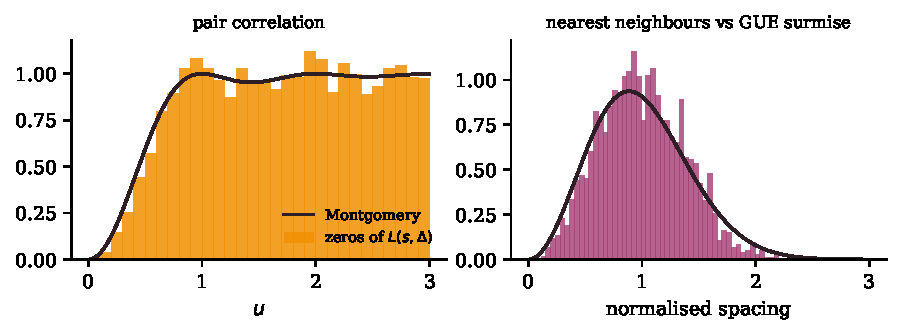
\includegraphics[width=\textwidth]{figs/delta_pair_correlation.pdf}
\caption{Zeros of $L(s,\Delta)$ with ordinates in $[500,2000]$ ($2495$ zeros, located as sign changes of $Z_\Delta$ on a grid of step $0.04$). Left: empirical pair correlation of the unfolded ordinates in bins of width $0.1$, against Montgomery's function $1-(\sin\pi u/\pi u)^2$. Right: histogram of the $2494$ normalised nearest neighbour spacings against the Wigner surmise $\frac{32}{\pi^2}s^2e^{-4s^2/\pi}$.}\label{fig:09bpair}
\end{figure}

\section{The field through the Thorin lens}\label{sec:09bthorin}

The chapters that follow reformulate $L(s,\Delta)$ in terms of a probability law, the P\'olya variable $W$ of Chapter~\ref{ch:10} with density $\Phi_\Delta(u)\propto\Delta(ie^u)e^{6u}$, its Thorin measure (Chapter~\ref{ch:10b}), and the extreme value variable $M^*$ of Chapter~\ref{ch:11}. Here we record what the results of this chapter say in that language. Everything in this section is an exact consequence of the cited theorems, and none of it is evidence for or against the Riemann hypothesis.

\begin{proposition}[Selberg's theorem as a statement about a characteristic function; this book]\label{prop:09bpolya}
Let $\varphi_W(t)=\E e^{itW}$. For real $t$,
\[
\log|L(6+it,\Delta)|=\log|\varphi_W(t)|-\log|\Gamma(6+it)|+\log\bigl(\Gamma(6)L(6,\Delta)\bigr),
\]
and, as $|t|\to\infty$,
\[
\log|L(6+it,\Delta)|=\log|\varphi_W(t)|+\frac\pi2|t|-\frac{11}2\log|t|+C_\Delta+O\Bigl(\frac1{|t|}\Bigr),
\]
with $C_\Delta=\log(120\,L(6,\Delta))-\frac12\log2\pi=3.6355$.
Consequently, under the hypothesis of Theorem~\ref{thm:09bselbergdelta}, for $t$ uniform on $[T,2T]$,
\[
\frac{\log|\varphi_W(t)|+\frac\pi2t-\frac{11}2\log t+C_\Delta}{\sqrt{\frac12\log\log T}}\Longrightarrow N(0,1).
\]
\end{proposition}

\begin{proof}
By Theorem~\ref{thm:ch10kernel}, $\varphi_W(t)=\Lambda(6+it,\Delta)/\Lambda(6,\Delta)$, and $|\Lambda(6+it,\Delta)|=(2\pi)^{-6}|\Gamma(6+it)||L(6+it,\Delta)|$, $\Lambda(6,\Delta)=(2\pi)^{-6}\Gamma(6)L(6,\Delta)$. This gives the identity. Stirling's formula $\log|\Gamma(\sigma+it)|=(\sigma-\frac12)\log|t|-\frac\pi2|t|+\frac12\log2\pi+O(1/|t|)$ at $\sigma=6$ gives the expansion, with $L(6,\Delta)=0.792123$. The last statement is Theorem~\ref{thm:09bselbergdelta} rewritten.
\end{proof}

The density $\Phi_\Delta$ extends analytically to the strip $|\operatorname{Im}u|<\frac\pi2$, since $ie^{u}$ stays in the upper half plane there, and it is this strip that forces $|\varphi_W(t)|$ to decay like $e^{-\pi|t|/2}$ up to powers of $t$. Under the Riemann hypothesis for $\Delta$, Proposition~\ref{prop:09bpolya} says that on top of this deterministic decay the characteristic function of an explicit, smooth, symmetric probability law carries lognormal fluctuations of variance $\frac12\log\log t$. By Theorem~\ref{thm:09brs} its real zeros, which are the zeros of $L(s,\Delta)$ on the critical line, have GUE correlations for test functions in the restricted range, and the heuristics of Section~\ref{sec:09blogcorr} predict that the maxima of $\log|L(6+it,\Delta)|$ over unit windows follow the Fyodorov Hiary Keating asymptotics. The same holds for the P\'olya kernel of the Riemann $\Xi$ function in Chapter~\ref{ch:10}, with the lognormal fluctuations unconditional by Theorem~\ref{thm:09bselberg} and, under the Riemann hypothesis for $\zeta$, Montgomery's theorem in place of Theorem~\ref{thm:09brs}.

Under the Riemann hypothesis for $\Delta$ the same function is a logarithmic potential. By Chapter~\ref{ch:10b} the function $s\mapsto\Lambda(6)/\Lambda(6+\sqrt s)$ is then the Laplace transform of the generalized gamma convolution $Y=\sum_kE_k/\gamma_k^2$, with $E_k$ independent standard exponentials and Thorin measure $\tau_\Delta=\sum_k\delta_{\gamma_k^2}$.

\begin{proposition}[The field as the potential of the Thorin measure; this book]\label{prop:09bpotential}
Assume the Riemann hypothesis for $L(s,\Delta)$, with zeros $6\pm i\gamma_k$, $\gamma_k>0$. For real $t\ne\pm\gamma_k$,
\[
\log|\varphi_W(t)|=\sum_k\log\Bigl|1-\frac{t^2}{\gamma_k^2}\Bigr|=\int_{(0,\infty)}\log\Bigl|1-\frac{t^2}{x}\Bigr|\,\tau_\Delta(dx)=-\log\bigl|\mathcal{L}_Y(t^2)\bigr|,
\]
where $\mathcal{L}_Y(u)=\prod_k(1-u/\gamma_k^2)^{-1}$ is the meromorphic continuation of the moment generating function $\E e^{uY}$, $u<\gamma_1^2$, to $\C$. Moreover, on each interval between consecutive zeros, $t\mapsto\log|\varphi_W(t)|$ is strictly concave.
\end{proposition}

\begin{proof}
Theorem~\ref{thm:ch10hadamard} gives $\Lambda(6+z)/\Lambda(6)=\prod_k(1+z^2/\gamma_k^2)$ for all $z$, with $\sum_k\gamma_k^{-2}<\infty$; put $z=it$ and take logarithms of absolute values, which is legitimate because the product converges absolutely. The integral is the same sum written against $\tau_\Delta$. For $u<\gamma_1^2$, independence gives $\E e^{uY}=\prod_k\E e^{uE_k/\gamma_k^2}=\prod_k(1-u/\gamma_k^2)^{-1}$, and the product converges to a meromorphic function of $u$ with simple poles at the $\gamma_k^2$. Finally $\frac{d^2}{dt^2}\log|1-t^2/\gamma^2|=-2(\gamma^2+t^2)/(\gamma^2-t^2)^2<0$, and a convergent sum of strictly concave functions is strictly concave.
\end{proof}

So, under the Riemann hypothesis, the field of this chapter is, after the archimedean drift, the logarithmic potential of the Thorin measure, evaluated at the point $t^2$ of the half line that carries the measure. The log correlated picture predicts that this potential, for atoms with sine kernel statistics, fluctuates like a log correlated Gaussian field; for random unitary matrices Hughes, Keating and O'Connell \cite{hko2001} proved that the logarithm of the characteristic polynomial along the circle converges, as a random generalised function, to such a field. The hybrid product also has a reading here, which we offer only as a heuristic: $Z_X$ involves the zeros within about $1/\log X$ of $t$, that is, the Thorin atoms within about $2t/\log X$ of $t^2$, while the potential of the far atoms is smooth in $t$ and is carried by the primes $p\le X$ through the explicit formula used in Chapter~\ref{ch:10d}. The prime and zero parts of $V_\Delta$ are then the variances of the far and near potentials.

The extreme value representation of Chapter~\ref{ch:11} is a third view of the same object. There $\Delta(iy)=e^{-2\pi y}F(y)$ with $F$ the distribution function of $M^*$, the maximum of the independent variables $E_{j,n}/(2\pi n)$, and $L(s,\Delta)=\E[Q(s,2\pi M^*)]$ (Theorem~\ref{thm:ch11main}). Proposition~\ref{prop:ch11posterior} there identifies $\Phi_\Delta$ as a conditional law; on the critical line it reads as follows.

\begin{proposition}[The critical line through $M^*$; this book]\label{prop:09bmstar}
Let $G$ have the gamma law of shape $6$ and unit rate, independent of $M^*$. For real $t$,
\[
\frac{\Gamma(6+it)}{\Gamma(6)}\,L(6+it,\Delta)=\E\bigl[G^{it}\,;\,G\ge2\pi M^*\bigr].
\]
The finite measure $\nu(B)=\Prob(\log G\in B,\ G\ge2\pi M^*)$ has total mass $L(6,\Delta)$ and equals $L(6,\Delta)$ times the law of $W+\log2\pi$.
\end{proposition}

\begin{proof}
Proposition~\ref{prop:ch11posterior}, with $G_6=G$, says that conditional on $\{G\ge2\pi M^*\}$, an event of probability $L(6,\Delta)$ by Theorem~\ref{thm:ch11main}, the variable $\log(G/2\pi)$ has density $\Phi_\Delta$, which gives the second statement. At $z=it$ the proposition yields $\E[(G/2\pi)^{it};G\ge2\pi M^*]=L(6,\Delta)\Lambda(6+it,\Delta)/\Lambda(6,\Delta)$, and $\Lambda(s,\Delta)=(2\pi)^{-s}\Gamma(s)L(s,\Delta)$ turns this into the first.
\end{proof}

So the P\'olya variable is the logarithm of a gamma variable conditioned to beat $2\pi M^*$, recentred. Two kinds of extremes should not be confused here. The variable $M^*$ is a maximum of independent exponentials on the Mellin side, and it determines $L(s,\Delta)$ for every $s$; the maxima of $\log|L(6+it,\Delta)|$ over unit windows, the analogue for $\Delta$ of Conjecture~\ref{conj:09bfhk}, are maxima of a log correlated field on the spectral side. Proposition~\ref{prop:09bmstar} writes $L(6+it,\Delta)$ as the Fourier transform of a measure built from $G$ and $M^*$, but we see no direct route from the law of $M^*$ to those maxima beyond the decay rate of Proposition~\ref{prop:09bpolya}.

\section{Notes}

Arguin, Belius and Harper~\cite{abh2017} first proved the two leading terms of Conjecture~\ref{conj:09bfhk} for a randomised model of $\zeta$, and the proofs for $\zeta$ itself collected in Theorem~\ref{thm:09bfhkproved} adapt the branching random walk methods behind Theorem~\ref{thm:09bbrw}.

Our own contributions are modest and labelled: Proposition~\ref{prop:09blefttail} (an elementary fact we use to explain the left tail), Proposition~\ref{prop:09bcov} (the covariance of the random model, a standard computation written out), Proposition~\ref{prop:09bballot} (the ballot computation in a model where it is exact), Conjecture~\ref{conj:09bvar} (the CFKRS and hybrid heuristics written out for $\Delta$, with the constant $A_\Delta$ computed), and the three propositions of Section~\ref{sec:09bthorin}. Proposition~\ref{prop:09bks} is Keating and Snaith's, in our presentation. All data in this chapter come from our PARI/GP and Python computations: the $50{,}000$ values of $\log|L(6+it,\Delta)|$, the $2000$ window maxima, the $2495$ zeros, the random field and the Steinhaus simulations, and the constants $A_\zeta$, $A_\Delta$, $B_\Delta$.

\section{Exercises}

\begin{enumerate}
\item\label{ex:09bcumulants} Using Proposition~\ref{prop:09bks}, compute $\kappa_5(\infty)$ and $\kappa_6(\infty)$ for $\log|\Lambda_N|$, and show that $(-1)^j\kappa_j(\infty)>0$ for all $j\ge3$. Deduce that, in standard units, the skewness of $\log|\Lambda_N|$ is asymptotic to $-\frac{\pi^2}4\bigl(\frac12\log N\bigr)^{-3/2}$. Compare with the data of Section~\ref{sec:09btail}.
\item\label{ex:09bmertens} Using $L(s,\Delta\times\Delta)=\zeta(s)L(s,\Sym^2\Delta)$ and the prime number theorem for $\Sym^2\Delta$, prove that
\[
A_\Delta=\log L(1,\Sym^2\Delta)-\sum_p\sum_{m\ge2}\Bigl(\frac1m-\frac1{m^2}\Bigr)\frac{(2\cos m\theta_p)^2}{p^m},
\]
and show that the analogous identity for $\zeta$ reads $A_\zeta=-\sum_p\sum_{m\ge2}(\frac1m-\frac1{m^2})p^{-m}$. Check numerically that $A_\zeta=-0.1762$ using the primes below $10^4$.
\item\label{ex:09bbridge} Prove that a Brownian bridge of variance $\sigma^2$ per unit time from $0$ to $e$ on $[0,n]$ stays below $h>\max(0,e)$ with probability $1-\exp(-2h(h-e)/(\sigma^2n))$. Using Proposition~\ref{prop:09bballot}, find $m_n$ for the $b$ ary tree with $\sigma^2=\frac12\log b$ and check that $cn$ and $\theta$ do not depend on $b$ when $n$ is measured in units of $\log b$.
\item\label{ex:09bfour} (Probabilistic.) For the Steinhaus model show that $\E|S(x)|^4$ equals the number of quadruples $(n_1,n_2,n_3,n_4)$ in $[1,x]^4$ with $n_1n_2=n_3n_4$, and that this is $\asymp x^2\log x$. Explain why this shows that $S(x)/\sqrt x$ is not asymptotically Gaussian, and why it is consistent with Theorem~\ref{thm:09bharper} by H\"older's inequality.
\item\label{ex:09bharper} Prove Lemma~\ref{lem:09bplancherel} in detail, and use it with $f(n)=1$ to show that for $\sigma>1$
\[
\int_1^\infty\frac{\lfloor u\rfloor^2}{u^{1+2\sigma}}\,du=\frac1{2\pi}\int_{-\infty}^\infty\frac{|\zeta(\sigma+it)|^2}{|\sigma+it|^2}\,dt .
\] Evaluate both sides asymptotically as $\sigma\to1^+$.
\item\label{ex:09bconcave} Assume the Riemann hypothesis for $\Delta$. Using Propositions~\ref{prop:09bpolya} and \ref{prop:09bpotential}, show that between two consecutive zeros $\gamma_k<\gamma_{k+1}$ the function $\log|L(6+it,\Delta)|$ has exactly one critical point once $\gamma_k$ is large enough. (Hint: compare the second derivative of the archimedean term with that of the potential, and use that the gaps $\gamma_{k+1}-\gamma_k$ are bounded, by the counting formula of Section~\ref{sec:09bpair}.)
\end{enumerate}

\section{Open computational problems}

\begin{compproblem}[Selberg's theorem and the hybrid constant at height $10^8$]\label{cp:09bselberg}
Objective: test Conjecture~\ref{conj:09bvar} and the cumulant predictions of Proposition~\ref{prop:09bks} for $L(s,\Delta)$ at heights where $\frac12\log\log T$ has moved appreciably. Objects and scale: $\log|L(6+it,\Delta)|$ on grids of spacing $0.01$ in windows of length $10^4$ centred at $T=10^4,10^5,10^6,10^7,10^8$ (about $10^6$ values per window), and $A_\Delta$ to five digits, from $\tau(p)$ for all $p\le10^9$ or, more cheaply, from the identity of Exercise~\ref{ex:09bmertens} with $L(1,\Sym^2\Delta)=\frac{\pi}{2}\frac{(4\pi)^{12}}{11!}\langle\Delta,\Delta\rangle$, where $\langle\Delta,\Delta\rangle=\int_{\SL_2(\Z)\backslash\mathbb H}|\Delta(\tau)|^2y^{12}\,dx\,dy/y^2$ is computed by PARI/GP \texttt{mfpetersson}. Route: an Odlyzko Sch\"onhage type multi evaluation \cite{odlyzkoschonhage1988} of the approximate functional equation for $\Delta$, or interval arithmetic in the style of Platt for certified values, checked against PARI/GP \texttt{lfun}. Deliverable: a table of sample variance, $\kappa_3$, $\kappa_4$ and their standard errors (by block bootstrap over zero spacings) against $V_\Delta(T)$ and $\kappa_j(\infty)$; and a fit of the residual $\operatorname{Var}-V_\Delta(T)$ against $1/\log T$. Why it matters: it would show whether the agreement found at $T\approx1500$ persists, and measure the lower order terms that the hybrid heuristic leaves out.
\end{compproblem}

\begin{compproblem}[The law of the maximum]\label{cp:09bmax}
Objective: estimate the distribution of $M_T-m_T$ (Theorem~\ref{thm:09bfhkproved}) for $\zeta$ and for $L(s,\Delta)$ and compare it with a randomly shifted Gumbel law. Objects and scale: $10^5$ unit windows at each of the heights $10^{10}$, $10^{16}$, $10^{22}$ for $\zeta$ and $10^5$ windows at heights up to $10^8$ for $\Delta$; in parallel, $10^6$ realisations of the Steinhaus and Sato Tate random Euler products and of a matched branching random walk, recording its derivative martingale. Route: for $\zeta$ and $\Delta$, Odlyzko Sch\"onhage multi evaluation \cite{odlyzkoschonhage1988} (for $\zeta$, also Hiary's fast algorithms) on fine grids with local refinement of maxima; for the models, GPU evaluation of truncated Euler products, and a fit of $\Prob(M\le y)$ to $\E\exp(-C^*D_\infty e^{-2y})$. Deliverable: empirical distribution functions of $M_T-m_T$, estimates of the additive constants for $\zeta$, $\Delta$ and the models, tail plots of $\log\Prob(M>y)+2y-\log y$, and a test of the shape $ye^{-2y}$. Why it matters: the limit law is the open part of Conjecture~\ref{conj:09bfhk}.
\end{compproblem}

\begin{compproblem}[Pair correlation and spacings for $\Delta$ to height $10^7$]\label{cp:09bpair}
Objective: measure the finite height corrections to the GUE statistics of the zeros of $L(s,\Delta)$. Objects and scale: all zeros with $0<\gamma\le10^5$, about $2.8\times10^5$, certified by Turing's method, and blocks of $10^5$ consecutive zeros near $\gamma=10^6$ and $10^7$. Route: PARI/GP \texttt{lfunzeros} or Rubinstein's \texttt{lcalc}, with a dense search near small gaps to recover close pairs; the Bogomolny Keating formula \cite{bogomolnykeating1996} adapted to $\Delta$, and spacing laws of small unitary matrices from Fredholm determinants. Deliverable: pair correlation residuals against $1-(\sin\pi u/\pi u)^2$ with error bands, the spacing variance as a function of height against $0.180$, and the effective matrix size for $\Delta$ that best fits the spacing law at each height, compared with the analogue of the prediction of \cite{bblm2006}. Why it matters: it would show whether finite height effects account for the narrow spacing law (variance $0.138$) observed near $t\approx10^3$, and test the arithmetic corrections in degree two.
\end{compproblem}

\begin{compproblem}[Harper's constant and critical chaos]\label{cp:09bharper}
Objective: estimate the limit of $c(x)=\E|S(x)|(\log\log x)^{1/4}/\sqrt x$ for the Steinhaus model, which exists by the theorem of Gorodetsky and Wong (Section~\ref{sec:09bharper}), and the speed of convergence; decide numerically whether $c(x)$ converges for the Rademacher model; and relate the limits to critical chaos. Objects and scale: $10^4$ realisations of each model with $x$ up to $10^{10}$, and for each realisation the total mass $\int_{-1/2}^{1/2}|F_x(\frac12+\frac1{\log x}+it)|^2dt$ of the truncated Euler product over $p\le x$. Route: segmented sieves on GPUs generating $f(n)$ from random values at primes; variance reduction by conditioning on the small primes. Deliverable: plots of $c(x)$ with confidence bands; the joint law of $S(x)/\sqrt x$ and the chaos mass, with a test of the conditional Gaussian picture of Section~\ref{sec:09bharper}; and the same for the character sums of \cite{harper2023} with $r$ prime near $10^{12}$. Why it matters: Harper's theorem gives the order of magnitude but not a constant, and we know of no closed form for the limit of $c(x)$; a numerical value of the limit, its rate of approach, and its relation to the critical measure would indicate what the next theorem should be.
\end{compproblem}
